\section{Einführung und Überblick}

\begin{definition}{Software Engineering}
\begin{itemize}
    \item Disziplinen: Anforderungen, Architektur, Implementierung, Test und Wartung.
    \item Ziel: Strukturierte Prozesse für Qualität, Risiko- und Fehlerminimierung.
\end{itemize}
\end{definition}

\begin{definition}{Modellierung in der Softwareentwicklung}
\begin{itemize}
    \item Modelle als Abstraktionen: Anforderungen, Architekturen, Testfälle.
    \item Einsatz von UML: Skizzen, detaillierte Blueprints, vollständige Spezifikationen.
    \end{itemize}
\end{definition}

\begin{definition}{Wrap-up und Ausblick}
\begin{itemize}
    \item Solide Analyse- und Entwurfskompetenzen sind essenziell.
    \item Iterativ-inkrementelle Modelle fördern agile Entwicklung.
    \item Nächste Lerneinheit: Detaillierte Anforderungsanalyse.
\end{itemize}
\end{definition}

\section*{1 Vorlesung 01}
1.1 Charakteristiken von Wasserfall, iterativ-inkrementellen und agilen Softwareentwicklungsprozessen\\
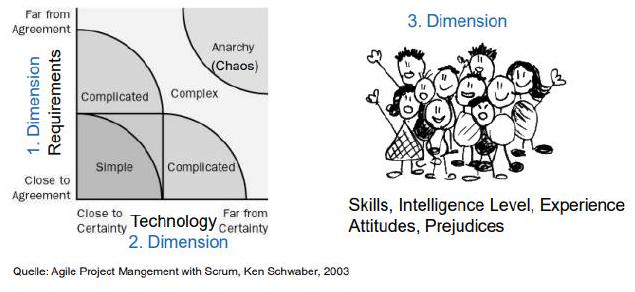
\includegraphics[max width=\textwidth, center]{2024_12_29_0d1d7b5551ea1b4b41bdg-01}

Abbildung 1: Klassifizierung Software-Entwicklungs-Probleme

\section*{Prozesse im Softwareengineering Kernprozesse}
\begin{itemize}
  \item Anforderungserhebung
  \item Systemdesign/technische Konzeption
  \item Implementierung
  \item Softwaretest
  \item Softwareeinführung
  \item Wartung/Pflege
\end{itemize}

\section*{Unterstützungsprozesse}
\begin{itemize}
  \item Projektmanagement
  \item Qualitätsmanagement
  \item Risikomanagement
\end{itemize}

Begriffe Warum wird modelliert: Um Analyse- und Designentwürfe zu diskutieren, abstimmen und zu dokumentieren bzw. zu kommunizieren. Modell: Ein Modell ist ein konkretes oder gedankliches Abbild eines vorhanden Gebildes oder Vorbild für ein zu schaffendes Gebilde (hier Softwareprodukt).\\
Original: Das Original ist das abgebildete oder zu schaffende Gebilde.\\
Modellierung: Modellierung gehört zum Fundament des Software Engineerings

\begin{itemize}
  \item Software ist vielfach (immer?) selbst ein Modell
  \item Anforderungen sind Modelle der Problemstellung
  \item Architekturen und Entwürfe sind Modelle der Lösung
  \item Testfälle sind Modelle des korrekten Funktionierens des Codes usw.\\
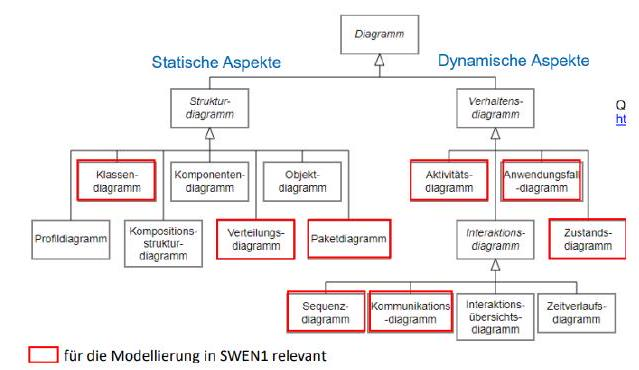
\includegraphics[max width=\textwidth, center]{2024_12_29_0d1d7b5551ea1b4b41bdg-01(1)}
\end{itemize}

Abbildung 2: Diagramme UML Übersicht

\subsection*{1.1.1 Code and Fix}
Vorgehen, bei dem Codierung oder Korrektur im Wechsel mit Ad-hoc-Tests die einzigen bewussten ausgeführten Tätigkeiten der Software-Entwicklung sind: Schnell, Agil, Einfach am Anfang, Schlecht Planbar, Schlecht Wartbar, Änderungen s. Aufwändig

\subsection*{1.1.2 Wasserfallmodell}
Die Software-Entwicklung wird als Folge von Aktivitäten/Phasen betrachtet, die durch Teilergebnisse (Dokumente) gekoppelt sind. Die Reihenfolge der Ak-\\
tivitäten ist fest definiert. : gut planbar, klare Aufteilung in Phasen, Schlechtes Risikomanagment, nie alle Anforderungen zu Anfang bekannt

\subsection*{1.1.3 Iterativ-inkrementelle Modelle}
Software wird in mehreren geplanten und kontrolliert durchgeführten Iterationen schrittweise (inkrementell) entwickelt: Flexibles Modell, Gutes Risikomanagement, Frühe Einsetzbarkeit, Planung upfront hat Grenzen, Kunde Involviert über ganze Entwicklung

Agile Softwareentwicklung Basiert auf interativ-inkrementellen Prozessmodell, Fokussiert auf gut dokumentierten und getesteten Code statt auf ausführlicher Dokumentation

\subsection*{1.2 Zweck und den Nutzen von Modellen in der Softwareentwicklung}
\begin{itemize}
  \item Modell von Requirements (close to/ far from Agreement) \& Technology (known / unknown)\\
Ein Modell ist ein konkretes oder gedankliches Abbild eines vorhanden Gebildes oder Vorbild für ein zu schaffendes Gebilde (hier Softwareprodukt).
\end{itemize}

\subsection*{1.2.1 Unified Modelling Language (UML)}
UML ist die Standardsprache für die graphische Modellierung von Anforderungen, Analyse und Entwürfen im Software Engineering (objektorientierte Modellierung). (As a sketch, blueprint, programminglanguage)

\subsection*{1.3 Artefakte in einem iterativinkrementellen Prozess illustrieren und einzuordnen}
\begin{center}
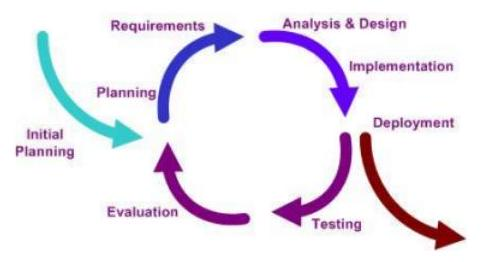
\includegraphics[max width=\textwidth]{2024_12_29_0d1d7b5551ea1b4b41bdg-02(1)}
\end{center}

Abbildung 3: Incremental Model